De NOT\index{NOT} werkt als een inverter\index{Inverter}. Dus als er een 1 op de ingang wordt aangeboden dan staat er een 0 op de uitgang en omgekeerd. De waarheidstabel voor de inverter is dus heel eenvoudig:

\rowcolors{2}{gray!10}{gray!20}
\begin{tabular}{ |c|c| }
\hline
\rowcolor{gray!60}
Input & Output \\
\hline
0 & 1 \\
\hline
1 & 0 \\
\hline
\end{tabular}


Het symbool voor de NOT is weergegeven in figuur \ref{symbool:not}

\begin{figure}[h]
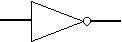
\includegraphics{inverter_symbool}
\centering
\caption{Symbool van een NOT}
\label{symbool:not}
\end{figure}

De NOT wordt gebouwd door gebruik van een enkele transistor en een weerstand (figuur \ref{circuit:not}.

\begin{figure}[h]
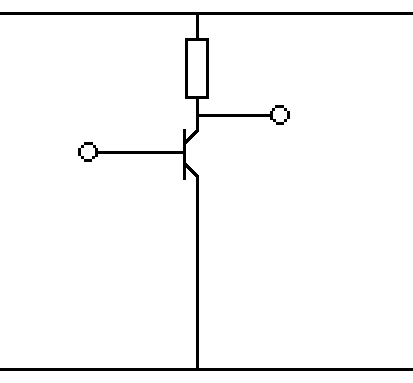
\includegraphics{inverter_circuit}
\centering
\caption{NOT circuit}
\label{circuit:not}
\end{figure}

